
\graphicspath{ {figures/ratio/} }

%CONTRIBUTIONS
%%%%%%%%%%%%%%%%%%%%%%%%%%%%%%%%%%%

\chapter{Ratiometric control of a transit to differentiation}
\label{ch:ratio}

A manuscript resembling this chapter was coauthored with Jean-Francois Boisclair Lachance, Nicol\'{a}s Pel\'{a}ez, Rachael Bakker, Heliodoro Navarro, Lu\'{i}s Amaral, Neda Bagheri, Ilaria Rebay, and Richard Carthew. A preprint is publicly available at \url{https://doi.org/10.1101/430744}. All of the experiments were conceived, designed, and executed by my colleagues. My contributions include all of the computational analysis and modeling and figures. I also wrote most of the the text under the guidance of Professor Richard Carthew.

%RATIO
%%%%%%%%%%%%%%%%%%%%%%%%%%%%%%%%%%%

\section{Background on the coordination of cell fate decisions}

Organismal development proceeds through a sequence of transitions that yield increasingly specific cellular states. Developmental programs employ a variety of strategies to coordinate transitions, ultimately ensuring that cells adopt the correct state in space and time. Elucidating these decision mechanisms is crucial to understanding the processes that guide development, as well as the diseases that arise when they fail.

How cells dynamically integrate the activities of one or more transcription factors to reliably execute state transitions is a long-standing question. Transcription factors initiate and enforce transitions by differentially regulating the expression of specific target genes \cite{Zheng1997,Ducy1997,McGhee2009}. Coordination among transcription factors can thus broaden the spectrum of possible cell responses to developmental cues \cite{ORiordan1999,Evans2003}. Positive and negative feedback can create bi-stable patterns of mutually exclusive transcription factor expression or activity that render state transitions irreversible \cite{Melen2005,Kueh2013,Yao2008,Park2012}. Cells can also regulate state transitions by differentially partitioning transcription factors between daughter cells \cite{Wolff2018}. In all of these models, mRNA and protein expression are believed to depend upon the absolute concentrations of the transcription factors involved \cite{Tontonoz1994,Laslo2006,Raj2010,Niwa2000}.

Studies of intercellular signaling suggest cells are capable of sensing relative levels of signaling molecules. For example, the TGF-$\beta$ pathway elicits a cell response following changes in input signaling relative to the preceding background \cite{Frick2017}. Fold-change, rather than absolute levels of $\beta$-catenin, dictate Wnt signal transduction in eukaryotic cells \cite{Goentoro2009a}. Likewise, aggregation of the social amoeba \textit{Dyctiostellium} depends on fold-change detection of extracellular cAMP concentrations \cite{Kamino2017}. Relative measurements can also involve multiple molecular components. In the BMP pathway, cells interpret multi-ligand inputs based on the relative levels of each ligand pair, with additive, differential, and ratiometric response types arising directly from the relative competition between different ligand-receptor pairs \cite{Antebi2017}. In yeast, pheromone response is insensitive to the absolute abundance of the G‐protein‐coupled receptor Ste2. Instead, cells respond to the fractional occupancy of the signal receptor by forming a ratiometric sensor between Ste2 and its regulatory inhibitor Sst2 \cite{Bush2016}. Topological features of molecular interaction networks, such as feed-forward loops, can also sense relative changes in molecule abundance \cite{Goentoro2009,Adler2018}. Combining such circuits with precise coordination of signaling inputs would yield a molecular decision mechanism that is robust to fluctuations in the abundance of participating molecules. Notably, while relevant transcription factors are precisely controlled during development \cite{Doe2017,Erclik2017}, it remains unknown whether cells sense the relative concentrations or activities of different transcription factors when executing cell state transitions.

Two ETS-domain transcription factors, the activator Pointed (Pnt) and the repressor Yan (also known as Anterior open, Aop), are essential regulators of cell fate transitions at numerous stages of \textit{Drosophila} development \cite{Gabay1996,Halfon2000,Morimoto1996,Xu2000,Flores2000}. Consistent with their opposing regulatory effects, genetic studies have shown that Pnt and Yan can act antagonistically in guiding numerous cell fate transitions \cite{Brunner1994,ONeill1994a,Gabay1996,Halfon2000}. The \textit{pnt} locus encodes two protein isoforms, PntP1 and PntP2, that differ in their N-terminal transactivation domains but share the same DNA-binding domain (Fig. \ref{fig:ratio:fig1}A) \cite{Klambt1993,Scholz1993}. Specifically, PntP1 is constitutively active whereas PntP2 requires phosphorylation via the RTK signaling pathway to become a potent activator \cite{ONeill1994a,Brunner1994}. Because both Pnt isoforms and Yan bind to a common ETS-binding DNA sequence motif GGA(A/T) \cite{Wei2010}, competition for occupancy and regulation of common target genes must be precisely orchestrated \cite{ONeill1994a,Halfon2000,Flores2000,Xu2000,Webber2013,Webber2013a,BoisclairLachance2018,Webber2018}.

Pnt and Yan display mutually exclusive expression patterns in several developing tissues \cite{BoisclairLachance2014}. The embryonic ventral ectoderm provides a classic example in which cells unambiguously reside in one of two stable states \cite{Gabay1996,Melen2005}. These and similar observations inspired a bistable switch model of cell fate specification in which the multipotent state is defined by high absolute Yan levels and the differentiated state is defined by high absolute Pnt levels \cite{Graham2010}. The model posits that RTK signaling triggers a transition from target gene repression to activation by degrading Yan and activating PntP2 \cite{Brunner1994,Rebay1995}. A positive feedback loop in which transient phosphorylation of PntP2 activates expression of \textit{pntP1} is thought to stabilize the transition by enabling prolonged signaling-independent stimulation of target genes \cite{Shwartz2013}. Sustained PntP1 expression in cells devoid of Yan thereby recapitulates a complementary expression pattern under the control of RTK signaling \cite{BoisclairLachance2014}. However, Pnt and Yan are also co-expressed during cell fate commitment in several developmental contexts \cite{BoisclairLachance2014}. For example, the two proteins are co-expressed in posterior follicle cells of the early egg chamber and throughout the embryonic mesoderm \cite{BoisclairLachance2014}, where they are required for specification of cell fates \cite{Morimoto1996,Halfon2000}. Co-expression also occurs in the larval eye \cite{BoisclairLachance2014}, despite the repeated use of RTK signaling to designate cell fates \cite{Freeman1996}. Eye development thus prompts exploration of how state transitions are resolved from concurrent Pnt and Yan expression in response to signaling cues.

Eye development is divided into two distinct phases, growth and differentiation. In the first phase, multipotent progenitor cells in the eye-field asynchronously proliferate from the earliest larval stage until the third instar stage of larval life \cite{Wolff1993}. The differentiation phase of eye development begins in the early third instar larva, when cells situated at the posterior margin of the eye disc start to differentiate into photoreceptor (R) cells, followed by progressively more anterior cells (Fig. \ref{fig:ratio:fig1}B). This wave of differentiation is initiated and coordinated by a morphogenetic furrow (MF), which traverses the eye disc from posterior to anterior for the remainder of the third instar stage up to the early pupal stage \cite{Voas2004}. Progenitor cells located immediately anterior to the MF arrest in G1 of the cell cycle and express a transcription factor called Atonal. Refinement of Atonal expression within this field establishes the differentiation program by specifying individual R8-type photoreceptors in a periodic pattern immediately posterior and parallel to the MF \cite{Jarman1994,Zhang2006}. Each R8 cell then locally secretes an RTK ligand that induces R8's multipotent neighbors to differentiate into other photoreceptor types (Fig. \ref{fig:ratio:fig1}C) \cite{Freeman1996,Voas2004}. Transitions sequentially occur approximately every two hours to form R2/R5, R3/R4, R1/R6, and R7 photoreceptors \cite{Wolff1993}. Many cells remain as multipotent progenitors even after all R cell fates have been adopted. These cells will adopt other fates at later stages of eye development, with any surplus eliminated by apoptosis \cite{Wolff1991}.

R cell fate specification violates three central tenets of the bistable switch model. First, Pnt and Yan do not exhibit a mutually exclusive expression pattern during eye development. The two proteins are extensively co-expressed in both progenitor and differentiating cells within and posterior to the MF \cite{BoisclairLachance2014}. Second, transitioning cells do not originate in a stable high Yan state. We recently quantified Yan protein dynamics during larval and early pupal eye development \cite{Pelaez2015a}. In progenitor cells, Yan displays pulsatile dynamics in which protein levels rapidly increase as the MF passes and then gradually decay back to low initial values. Third, transitioning cells do not adopt a stable high Pnt state. Visual inspection of eye discs carrying a fluorescent reporter for Pnt expression suggest that Pnt levels decay on a timescale comparable to Yan in transitioning cells \cite{BoisclairLachance2014}. Despite their similar expression patterns, the two proteins still exhibit antagonistic effects on R cell fate determination. Pnt stimulates progenitor cells to transit to an R cell fate while Yan inhibits these transitions \cite{ONeill1994a,Rebay1995}.

Here, we explore this apparent paradox to understand how two coexpressed transcription factors with comparable DNA binding specificity but opposing transcriptional functions elicit precisely controlled cell state transitions in the developing eye. We find that cell states are regulated by the relative abundance of these two proteins, rather than by their absolute concentrations. Progenitor cells dynamically maintain an approximately constant ratio of Pnt-to-Yan protein despite their absolute concentrations varying over time. Cells that transition to R cell fates rapidly increase their Pnt-to-Yan ratio, which remains elevated over time. We show that a ratio control strategy buffers this ratio against variable abundance of either protein. We also find that the signaling inputs of the Yan-Pnt network regulate the dynamics of the transcription factor ratio. Although Notch and Ras signals can both promote and inhibit differentiation in the developing eye \cite{Fortini1993,Freeman1996}, we find that Notch signaling predominantly decreases the Pnt-to-Yan ratio in progenitor cells while Ras signaling mainly increases the ratio. Notch and Ras signals thus inhibit and promote cell state transitions in the eye by dynamically tuning the ratio of the two transcription factors. We conclude that progenitor cells interpret an increase in the abundance of Pnt relative to Yan as a cue to differentiate.

\section{PntGFP expression dynamics in the developing eye }

Although Pnt expression has been qualitatively studied in the eye \cite{BoisclairLachance2014}, its dynamics have not been quantified. Therefore, we took advantage of a fully functional genomic transgene in which both \textit{pntP1} and \textit{pntP2} are C-terminally tagged with GFP. As previously reported \cite{BoisclairLachance2014}, \textit{pnt-gfp} rescues \textit{pnt} null mutants to viable, fertile adults with wild type external morphology (Fig. \ref{fig:ratio:figS1}A,B). Qualitative examination of Pnt-GFP expression in 100h eye-antennal imaginal discs revealed a region of very low expression in cells anterior to the MF, followed by strong expression in two parallel stripes of cells immediately posterior to the MF (Fig. \ref{fig:ratio:fig1}D, regions 1 and 2).

\begin{figure}[h!]
\centering
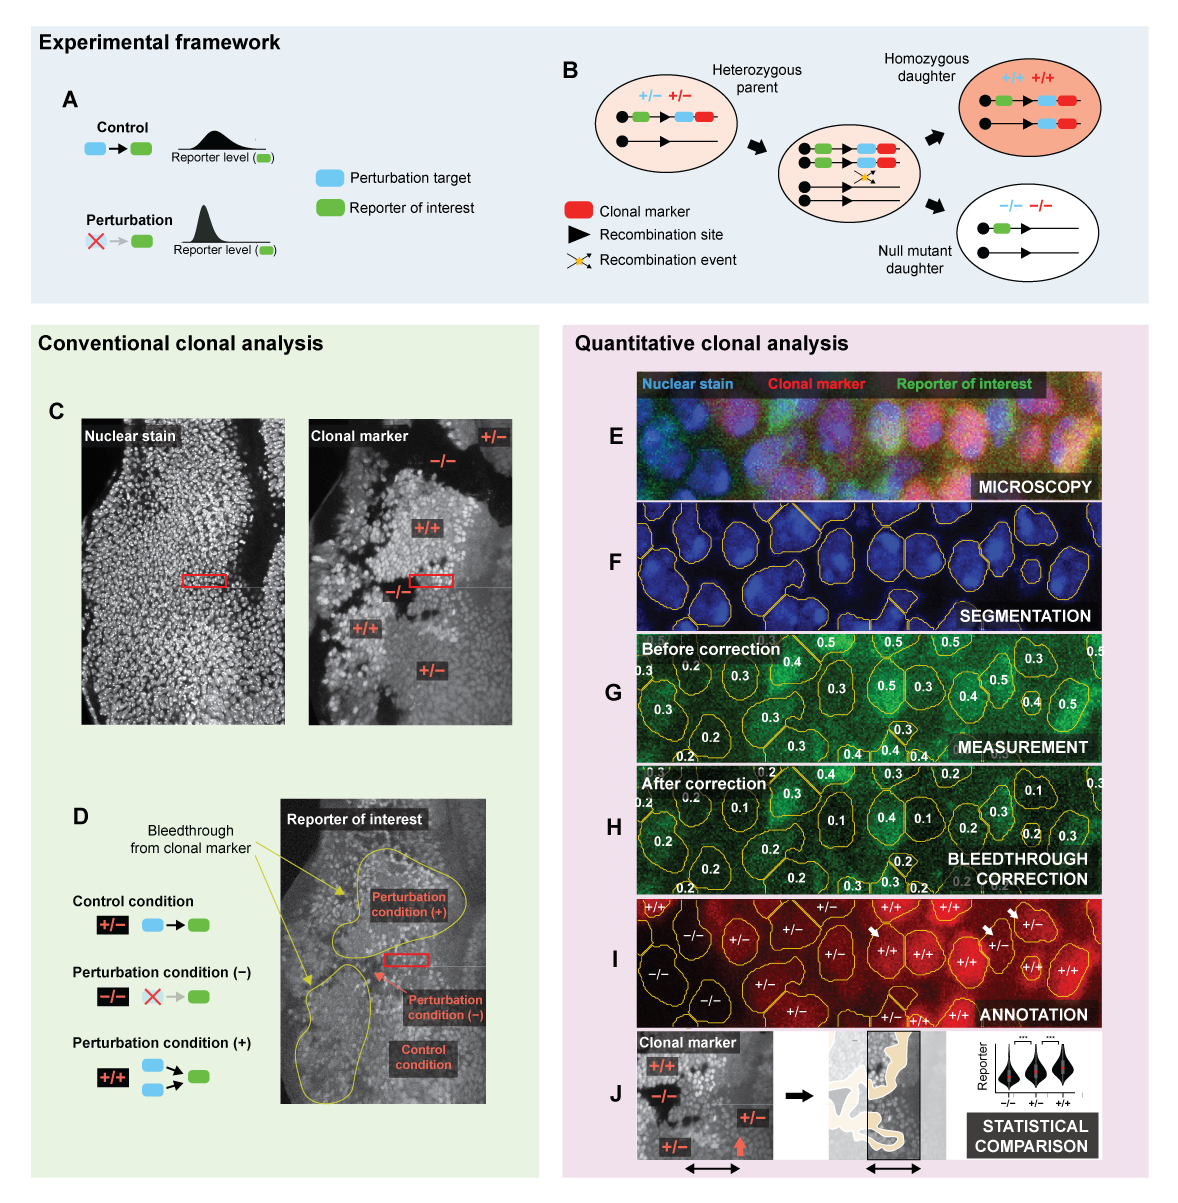
\includegraphics[width=1.0\columnwidth]{./figure_1}
\caption[Dynamics of Pnt and Yan expression during eye development.]{ (Continued on the next page.) }
\label{fig:ratio:fig1}
\end{figure}
\begin{figure}[h!]
\contcaption{\textbf{Dynamics of Pnt and Yan expression during eye development.} (A) Diagram of the \textit{pnt} locus encoding the Pnt-P1 and Pnt-P2 protein isoforms. The isoforms share an ETS DNA-binding domain (red) but are distinguished by the presence of a SAM domain (blue) within Pnt-P2. Green arrows at the C-termini depict insertion sites of GFP in the \textit{pnt-gfp} allele, black arrows at the N-termini depict insertion sites of the \textit{pnt\textsuperscript{HS20}} and \textit{pnt\textsuperscript{1277}} enhancer-trap alleles. Adapted from Shwartz et al. (2013). (B) Differentiation is initiated in the developing eye by the MF, which moves across the eye epithelium from posterior to anterior (white arrow). On the furrow's posterior side, G1-arrested progenitor cells differentiate (light blue). Formation of regularly spaced R8 photoreceptors (red dots) precedes recruitment of additional R cell types (yellow dots). On the anterior side, progenitor cells are still proliferating (dark blue). Axis refers to time elapsed since fertilization. Adapted from Pel\'{a}ez et al. (2015). (C) Top, cartoon of an apical view of the sequential differentiation of eight R cell types from multipotent progenitor cells (grey) and their relative positions within a single ommatidium. Arrows denote signals transmitted from the R8 to nearby cells. Bottom, a cross-section view through an eye disc, showing the epithelial constriction that marks the MF (boxed region) and then the relative nuclear positions of progenitors (grey) and specified R cells (various colors). Together, the stereotyped features depicted in this schematic enable unambiguous identification of each cell type as ommatidial assembly proceeds. Adapted from Pel\'{a}ez et al. (2015). (D) Maximum intensity projection of Pnt-GFP fluorescence in an imaginal disc fixed $\sim$ 100 h after fertilization. Right panel corresponds to the region enclosed by dashed white lines in the left panel. Morphogenetic furrow (orange arrow) precedes the first and second stripes of strong Pnt-GFP expression (black lines, labeled 1 and 2). (E) Pnt-GFP expression in progenitor cells. Grey points are individual cells, solid line is the smoothed moving average. Orange shading indicates the first and second stripes of Pnt-GFP expression. (F, G) R cell recruitment from the (F) first and (G) second pulses of Pnt-GFP expression. Solid lines and shaded regions denote moving averages and their 95\% confidence intervals. (H, I) Confocal images of (H) Pnt-P1 and (I) Pnt-P2 enhancer-trap co-expression with Pnt-GFP. Orientation is consistent with panel D. Morphogenetic furrow (orange arrow) precedes first and second stripes of Pnt-GFP induction (black lines, labeled 1 and 2). In merged images, Pnt-GFP is green and enhancer-trap expression is magenta. (J, K) Measured (J) Yan expression and (K) log\textsubscript{2}-transformed Pnt-GFP to Yan ratios in progenitor cells. Grey points are individual cells, solid line is a smoothed moving average.}
\end{figure}

\section{The Pnt-to-Yan ratio varies between cells in different states }

We used Histone-RFP fluorescence from a His2Av-mRFP transgene to label all eye cell nuclei for automated segmentation following direct fluorescence microscopy of fixed specimens \cite{Pelaez2015a,Pelaez2016}. Average Pnt-GFP fluorescence levels and exact 3D positions were then calculated for all nuclei in each developing eye disc. Pnt-GFP fluorescence levels were normalized to Histone-RFP, which provided some control over measurement noise and nuclear constriction that occurs at the MF \cite{Pelaez2015a,Pelaez2016}. We mapped each cell's position along the anterior-posterior coordinate of the eye disc to a point in developmental time. This linear approximation is sufficiently accurate because the MF moves across the eye field with approximately constant velocity, forming one column of R8 cells every two hours \cite{Basler1989,Campos-Ortega1977}. The distance between a cell and the MF is therefore proportional to the time elapsed since the MF passed. We also manually assigned a state value to each cell. Cell state classification is possible because nuclei can be unambiguously identified without cell-specific markers by their morphology, apical-basal position, and relative distance to the furrow \cite{Ready1976a,Tomlinson1985,Tomlinson1987a,Wolff1993,Pelaez2015a,Pelaez2016}. Combined, these data allowed us to infer a macroscopic view of cell state transition dynamics from the spatial arrangement of cells relative to each other and the MF. Although our approach cannot measure the developmental progression of an individual cell, it provides a dynamic view of thousands of cells across a developing eye. From this information, average cell behaviors can be reconstructed and modeled.

Progenitor cells anterior to the MF expressed a basal level of Pnt-GFP, but expression dramatically increased in cells immediately anterior to the MF (Fig. \ref{fig:ratio:fig1}E). This was followed by two successive pulses of Pnt-GFP expression, marked by peaks where protein expression reached maximal amplitude. The pulses matched the visual stripes seen in regions 1 and 2 (Fig. \ref{fig:ratio:fig1}D). Thereafter, Pnt-GFP decayed to a low basal level. The two pulses of Pnt-GFP in progenitor cells coincided with the two periods of transition to R cell states (Figs. \ref{fig:ratio:fig1}F,G and \ref{fig:ratio:figS1}C). Transitions to R8, R2/R5, and R3/R4 states occurred during the first pulse, while transitions to R1/R6, and R7 states occurred during the second pulse.

Based on prior description of the distinct temporal expression patterns of isoform-specific \textit{pnt} transcriptional reporters \cite{Shwartz2013}, we suspected that each pulse of Pnt-GFP corresponded to the induction of either PntP1 or PntP2. Using flies that carried the \textit{pnt-gfp} transgene and either a \textit{pntP1-} or \textit{pntP2}-specific reporter, we found that region 1 overlapped with the domain of strongest \textit{pntP1} reporter expression, and region 2 corresponded to the domain of strongest \textit{pntP2} reporter expression (Fig. \ref{fig:ratio:fig1}H,I). Low levels of \textit{pntP2} reporter expression were detected in region 1 and low levels of \textit{pntP1} reporter were detected in region 2. Therefore, Pnt expression appears as a PntP1-PntP2 pulse sequence. The two groups of differentiating R cells predominantly expressed PntP1 or PntP2 respectively (data not shown, see \cite{Pelaez2016}), suggesting that specific Pnt isoforms are used to specify distinct cell fates.

All cell state transitions coincided with a rapid increase in Pnt-GFP (Fig. \ref{fig:ratio:fig1}F,G). The earliest identified R cells had, on average, 25-50\% higher levels of Pnt-GFP than progenitor cells at comparable times. Pnt-GFP then rapidly decayed in all differentiating R cells, with all but the R7 cell type exhibiting faster decay kinetics than progenitor cells. Thus, transitioning R cells did not adopt stable high Pnt levels as predicted by a bi-stable model of R cell fate specification. Rather, the measured Pnt-GFP expression dynamics were similar to those previously reported for Yan \cite{Pelaez2015a}. Average levels of both proteins increased as the MF passed, then decayed during cell state transitions. These similar population-wide dynamics led us to ask how cell states are resolved from the co-expression of two transcription factors with opposing transcriptional functions at the single cell level.

We explored this question by simultaneously measuring Pnt-GFP and Yan in each nucleus using an anti-Yan monoclonal antibody. Previously, we had shown that Yan dynamics measured with the antibody were almost identical to those measured by a YFP tagged version of Yan \cite{Pelaez2015a}, validating our approach. Pnt-GFP and Yan were induced at the same time in progenitor cells (Figs. \ref{fig:ratio:fig1}E,J and \ref{fig:ratio:figS1}D). Yan levels reached a maximum amplitude between the two pulses of Pnt-GFP. Yan then decayed back to a basal steady-state level, interrupted by a transient plateau during the second pulse of Pnt-GFP. Despite their alternating maxima, the overall induction and decay of Pnt-GFP and Yan were concurrent in progenitor cells.

The similar dynamics prompted us to consider whether relative levels of Pnt and Yan dictate cell state transitions in the eye. To explore this possibility, we measured the ratio of Pnt-to-Yan in each progenitor cell. Strikingly, the average Pnt-to-Yan ratio remained dynamically stable about a constant value over time (Fig. \ref{fig:ratio:fig1}K). However, from 0 to 15 h, there was considerable cell-to-cell heterogeneity in the ratio. Some cells had above-average ratios when they were expressing peak levels of Pnt-GFP, and many cells had below-average ratios when they were between the Pnt-GFP pulses. After the second pulse of Pnt-GFP expression, cells acquired a slight bias towards Yan. These are the progenitor cells that remain multipotent and are used to differentiate into other cell types later in development \cite{Wolff1991}. As the two positive spikes in the ratio coincided with the two periods of cell state transition, we reasoned that dynamic changes in the ratio might control the state of cells and regulate their transit to differentiation.

As a first test of this idea, we quantified the levels of Pnt-GFP and Yan in cells that had undergone R cell state transitions. We focused on R2/R5 and R1/R6 cells, since they are representative of transitions of cells derived from groups 1 and 2, respectively. As previously noted, Pnt-GFP levels were elevated in both sets of ``young'' R cells as soon as we could confidently identify them (Fig. \ref{fig:ratio:fig2}A,B). In contrast, Yan levels were lower in these young R cells than in progenitor cells of comparable age (Fig. \ref{fig:ratio:fig2}C,D). This meant that the average ratio of Pnt-to-Yan was elevated 1.5- to 2-fold in young R cells (Fig. \ref{fig:ratio:fig2}E,F). The ratio elevation was more modest in young R2/R5 cells than in young R1/R6 cells, but all increases were significant (KS test, $p<0.001$). The elevated ratio persisted for all times thereafter as differentiation proceeded. Analogous ratio trends were evident with the other R cell types as well (Figs. \ref{fig:ratio:fig2}G and \ref{fig:ratio:figS2}), suggesting that different state transitions share a common requirement for sustained change in the Pnt-to-Yan ratio relative to progenitor cells (Fig. \ref{fig:ratio:figS2}C-G).

\begin{figure}[h!]
\centering
\vspace{0pt}
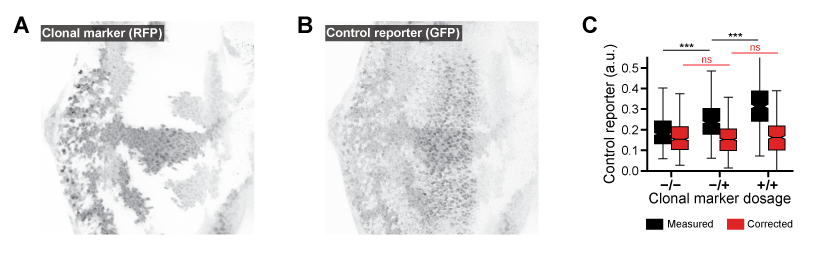
\includegraphics[width=1\columnwidth]{./figure_2}
\caption[Pnt-to-Yan ratios differ between cellular states.]{\textbf{Pnt-to-Yan ratios differ between cellular states.} (A-F) Measured (A, B) Pnt-GFP expression, (C, D) Yan expression, and (E, F) Pnt-GFP to Yan ratio dynamics in R2/R5 (blue) and R1/R6 (red) cells. Progenitors are grey. Solid lines are smoothed moving averages across 250 and 50 samples for progenitor and R cells, respectively. Yellow shading indicates time spanned by young R cells. (G) Comparison of Pnt-to-Yan ratio levels between young R cells (color filled boxes) and their concurrent progenitors (grey filled boxes). Colors denote R cell types. For each R cell type, the ten earliest identifiable R cells in each disc were designated as young R cells. Progenitor cells that fall within the time window spanned by these young R cells were designated as concurrent progenitors. Asterisks denote significance (KS 2-sample test, $p<0.001$). (H, I) Joint distributions of Pnt-GFP and Yan protein levels for young (H) R2/R5 and (I) R1/R6 cells. Progenitor cells concurrent with the corresponding young R cells are shown in grey. Black line denotes the median Pnt-to-Yan ratio among the progenitor cells shown.}
\label{fig:ratio:fig2}
\end{figure}

We next asked whether elevated Pnt-to-Yan ratios precede the onset of R cell state transitions. If R cells are recruited from a subpopulation of progenitors with relatively high ratios, some progenitors should exhibit ratios comparable to those of early R cells. We compared the distribution of Pnt-to-Yan ratios in young R cells versus concurrent progenitor cells (Fig. \ref{fig:ratio:fig2}H,I). The extensive overlap between the two populations implies that some cells we morphologically classified as progenitors were actually transitioning to R cell fates. Additionally, ratios may have increased among a subset of progenitors that did not ultimately transition to an R cell state. Many progenitors also adopted low Pnt-to-Yan ratios during this time period that did not overlap with the early R cell population. We reasoned that these cells were not viable candidates for recruitment, suggesting that the extent of variation in the ratio among progenitors constrains their competence for differentiation.

We then asked whether variation in the Pnt-to-Yan ratio strictly coincides with R cell fate transitions. We anticipated that variability should arise within the pool of progenitors from which R cells are recruited, then subside as fates are resolved. We previously reported methods to quantify the dynamic cell-to-cell heterogeneity of Yan concentration \cite{Pelaez2015a}. We applied similar analysis to simultaneously quantify the heterogeneity of Pnt, Yan, and the Pnt-to-Yan ratio among both progenitors and early R cells (Fig. \ref{fig:ratio:figS3}). A broad increase in variation of the ratio among progenitors coincided with the time periods in which state transitions occurred. Ratio variation was predominantly attributed to Yan and Pnt variability during the first and second groups of R cell state transitions, respectively. Heterogeneity among progenitors then decreased back to basal levels after all R cell fate transitions were complete. Similar trends were evident among transitioning R cells, but with a more rapid approach toward a consensus ratio following fate specification.

\begin{figure}[h]
\centering
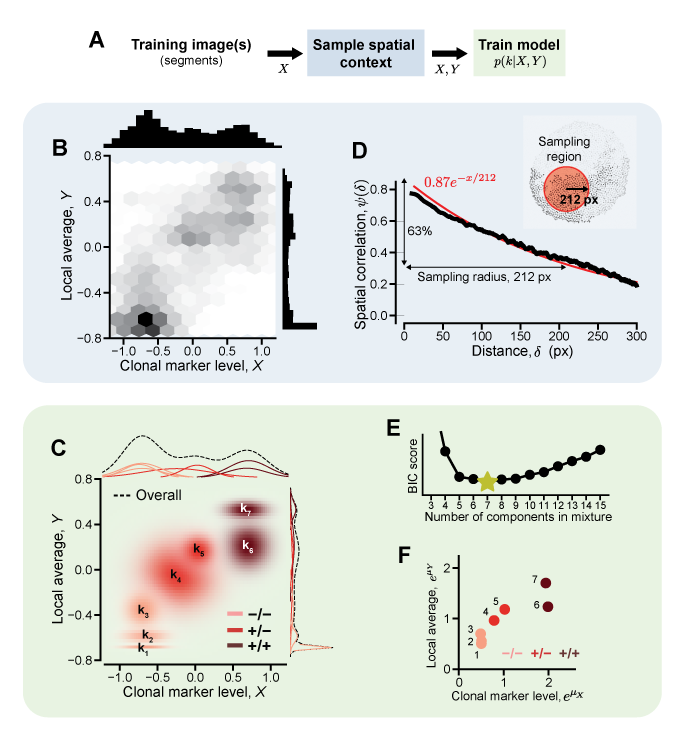
\includegraphics[width=1.0\columnwidth]{./figure_S3}
\caption[Dynamics of expression variability in progenitors and R cells.]{\textbf{Dynamics of expression variability in progenitor and R8, R2/R5 and R1/R6 cells.} Heterogeneities of (A) Pnt expression, (B) Yan expression, and (C) the log\textsubscript{2}-transformed ratio are estimated by de-trending fluctuations about a moving average of 250 sequential cells. Lines are moving averages of 250 sequential fluctuations, shaded regions are bootstrapped 95\% confidence intervals for the moving average. Colors denote cell type.}
\label{fig:ratio:figS3}
\end{figure}

\section{Cooperative DNA-binding sensitizes promoters to changes in Pnt-to-Yan ratio}

How could cells reprogram transcription in response to a change in the Pnt-to-Yan ratio across a wide range of absolute protein concentrations? Since both transcription factors have overlapping sequence specificity for DNA binding \cite{Xu2000,Halfon2000,Flores2000,Wei2010,Webber2013,Webber2013a,Nitta2015}, the underlying mechanism may be a natural consequence of competition for binding sites in target genes. To further explore this idea, we composed a simple equilibrium model in which two species, Yan ($Y$) and Pnt ($P$), competing for a finite pool of shared binding sites, $S$:
\begin{equation}
\begin{aligned}
Y + S &\xrightleftharpoons{\,K_{D,Yan}\,} SY \\
P + S &\xrightleftharpoons{\,K_{D,Pnt}\,} SP \\
\end{aligned}
\end{equation}
where $K_{D,Yan}$ and $K_{D,Pnt}$ are equilibrium association constants and $SY$ and $SP$ denote the bound species. Applying a mass balance to the total protein and binding site ($S_0$) abundances:
\begin{equation}
\begin{aligned}
Y_0 &= Y + SY \\
P_0 &= P + SP \\
S_0 &= S + SY + SP \\
\end{aligned}
\end{equation}
yields an analytically tractable system of nonlinear equations \cite{Wang1995}. Given a pair of absolute protein abundances $(Y_0,P_0)$, the Pnt binding site occupancy is simply $SP/S_0$. The phase diagram offered by this simple model suggests that if the sites are saturated, equilibrium occupancy by either factor is more sensitive to the relative concentration of the two factors than to the absolute concentration of both species (Fig. \ref{fig:ratio:figS4}A,B).

\begin{figure}[h]
\centering
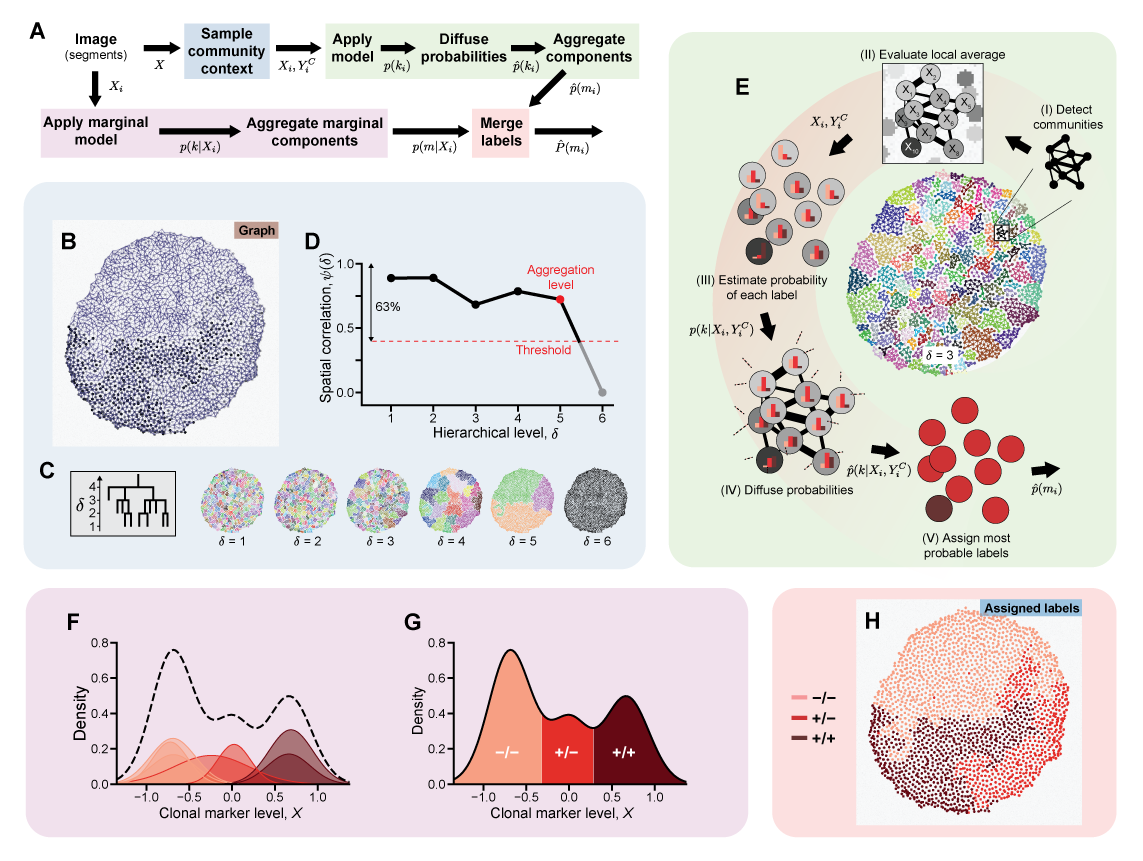
\includegraphics[scale=1.0]{./figure_S4}
\caption[Simple two-species competitive binding model]{\textbf{A simple two-species competitive binding model} (A) Model schematic. (B) Theoretical Pnt site occupancy as a function of transcription factor abundance. Equivalent binding affinities are used for illustrative purposes. Simultaneous proportional increases in absolute abundance of both species have minimal impact on Pnt occupancy, while varying ratio confers maximal change.}
\label{fig:ratio:figS4}
\end{figure}

However, the situation is more complex for Pnt and Yan. While there are several well-documented target genes that contain common binding sites for Pnt and Yan \cite{Halfon2000,Xu2000,Flores2000,BoisclairLachance2018}, Yan binds these enhancers with higher affinity than Pnt \cite{Xu2000}. Moreover, recent experiments suggest a scenario in which Pnt and Yan differentially interpret the structural syntax of \textit{cis}-regulatory modules \cite{BoisclairLachance2018}. This complex phenomenon is a consequence of cooperative recruitment between adjacent chromatin-bound Yan molecules. Yan monomers are able to polymerize via their sterile alpha motif (SAM) binding domains, enabling tightly-bound Yan monomers at strong ETS sites to stabilize the recruitment of additional Yan monomers to adjacent, weaker ETS sites or non-ETS sites \cite{Qiao2004,BoisclairLachance2018}. These cooperative effects could conceivably bias the competition between Pnt and Yan, which led us to consider a more complex model.

Hope, Rebay, and Reinitz recently introduced a modeling framework in order to probe the effects of \textit{cis}-regulatory syntax on Yan binding site occupancy \cite{Hope2017}. The model considers an ensemble of microstates, each defined by a unique configuration of vacant or Yan-bound sites. Each microstate is assigned a thermodynamic potential based on the cumulative influence of strong ETS-binding, weak non-ETS binding, and polymerization. We augmented this model by incorporating Pnt as a second transcription factor that competes for occupancy of the same binding sites (Fig. \ref{fig:ratio:figS5}A). 

Our formulation of the model is based on a single \textit{cis}-regulatory element consisting of $n$ adjacent binding sites, each of which may be designated as ETS or non-ETS. Each binding site may only exist in one of three binding states; bound by a single copy of Yan, bound by a single copy of Pnt, or unbound. Thermodynamic potentials are assigned to each binding state using two parameters for each transcription factor. The parameter $\alpha_X$ defines the free energy of transcription factor $X$ binding to an ETS site, while $\beta_X$ defines the free energy of binding to a non-ETS site (Fig. \ref{fig:ratio:figS5}A). A unique configuration of binding states for all $n$ binding sites constitutes a single microstate, $k$. The thermodynamic potential of each microstate is given by the superposition of thermodynamic potentials for each of its constituent binding sites. For each microstate, the stabilizing effect of polymerization is incorporated via a third parameter, $\gamma_X$, that defines the free energy of SAM-SAM binding between a pair of similar transcription factors bound to adjacent sites. The net result is a total thermodynamic potential, $\Delta G_k$, for each microstate. An example enumeration of all possible microstates for an element consisting of one ETS site preceding two non-ETS sites is provided in Figure \ref{fig:ratio:figS5}B. The statistical frequencies of each microstate are obtained via the canonical ensemble:
\begin{equation}
p_k = \frac{\displaystyle exp( \frac{-\Delta G_k}{RT} ) [P]^{a_P(k)}[Y]^{a_Y(k)} } {\displaystyle \sum_{k} {exp(\frac{-\Delta G_k}{RT})[P]^{a_P(k)}[Y]^{a_Y(k)}}}
\end{equation}
in which $p_k$ is the frequency of microstate $k$, $[P]$ and $[Y]$ are the Pnt and Yan concentrations, $a_P(k)$ and $a_Y(k)$ are functions representing the number of bound molecules of $P$ and $Y$ within microstate $k$, $T$ is a fixed temperature set to 300 K, and $R$ is the gas constant. Fractional occupancies for each binding site correspond to the cumulative frequency of all microstates in which the site is occupied by a given transcription factor. Overall fractional occupancies may then be computed by summing across all sites within the element.

\begin{figure}[h]
\centering
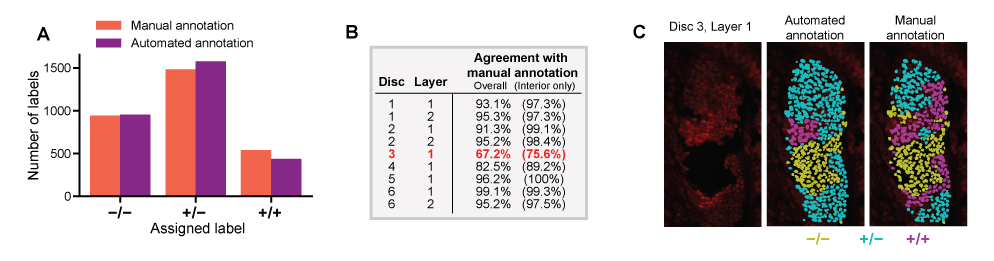
\includegraphics[width=0.9\columnwidth]{./figure_S5}
\caption[Thermodynamic model of transcription factor DNA binding.]{\textbf{Thermodynamic model of transcription factor DNA binding.} (A) Summary of thermodynamic interactions within one microstate of a cis-regulatory element containing one ETS site and two non-ETS sites. Solid black lines represent individual binding sites. Green and magenta rectangles denote Pnt and Yan molecules. Example thermodynamic potentials of strong ETS-binding, weak non-ETS binding, and polymerization interactions are denoted by $\alpha_{Pnt}$, $\beta_{Yan}$, and $\gamma_{Yan}$, respectively. For this microstate, $a_P(k)=1$ and $a_Y(k)=2$. (B) Enumeration of all possible microstates for a cis-regulatory element of length 3 in which only the first site carries the ETS designation. Solid black lines denote binding sites, green and magenta rectangles denote bound Pnt and Yan molecules. The cumulative thermodynamic potentials of each microstate, $\Delta G_k$, are listed beside each graphical depiction. Visual representation is adapted from \cite{Hope2017}. (C) Relative thermodynamic contributions of binding site affinity versus polymerization to microstate statistical frequencies as a function of Pnt and Yan concentration. For each point in the plane, influence of site affinity was calculated by weighting the sum of all ETS and non-ETS thermodynamic potentials for each microstate by the statistical frequency of the corresponding microstate. The influence of polymerization was analogously determined. The shown color scale reflects the relative magnitude of these two summations, normalized by limits of zero and complete polymerization.}
\label{fig:ratio:figS5}
\end{figure}

Using this model, we sought to characterize the sensitivity of Pnt binding site occupancy to changes in the Pnt-to-Yan ratio without neglecting cooperativity derived from \textit{cis}-regulatory syntax. We first considered a scenario in which Yan and Pnt did not exhibit cooperativity (Fig. \ref{fig:ratio:fig3}A). In the absence of stabilizing SAM-SAM interactions, the landscape of overall binding site occupancy is identical to that obtained with the simple binding model described above (Figs. \ref{fig:ratio:fig3}B and \ref{fig:ratio:figS4}B). Increasing the Pnt-to-Yan ratio revealed a gradual increase in Pnt occupancy for all individual binding sites (Fig. \ref{fig:ratio:fig3}C). This titration contour closely resembles a Langmuir isotherm or Michaelis-Menten saturation curve \cite{Fogler1987}.

We then introduced a stabilizing SAM-interaction for Yan (Fig. \ref{fig:ratio:fig3}D). The resultant landscape of overall Pnt binding site occupancy is clearly distinguished from the simple binding model by a sharpening of the transition from Yan to Pnt dominance in occupancy (Fig. \ref{fig:ratio:fig3}E). Weighting the energetic contributions of binding strength and polymerization by the statistical frequency of each microstate revealed that the transition is driven by an abrupt change in the dominant binding mechanism. Polymerization effects dominate binding site occupancy when the Pnt-to-Yan ratio is low, while binding strength dominates when the ratio is high (Fig. \ref{fig:ratio:figS5}C).

Increasing the Pnt-to-Yan ratio revealed nonlinear transitions from low to high Pnt occupancy for each individual binding site (Fig. \ref{fig:ratio:fig3}F). These transitions resemble Hill functional forms \cite{Fogler1987}, indicating the emergence of sharp thresholds that delimit distinct regimes of transcriptional output. At low Pnt-to-Yan ratios, Yan is able to polymerize and occupies all binding sites. At some critical Pnt-to-Yan ratio, Pnt-bound sites intersperse Yan-bound sites such that Yan is no longer able to polymerize. Pnt then out-competes Yan as the ratio increases further. These results recapitulate the long-standing notion that cooperative DNA-binding sensitizes transcriptional output to changes in transcription factor activity.

Assuming binding sites are saturated, then relative occupancy by Pnt and Yan is agnostic to changes in the absolute abundance of either factor, as long as the Pnt-to-Yan ratio remains constant. This mechanism, coupled with cooperativity, would enable modest changes in the Pnt-to-Yan ratio to elicit large changes in DNA binding site occupancy by either factor, and presumably large changes in mRNA synthesis given the opposing transcriptional effects of Yan and Pnt.

\begin{figure}[h!]
\centering
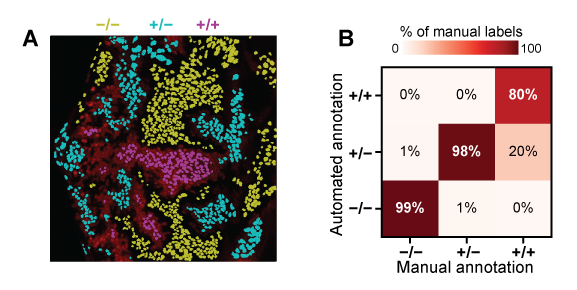
\includegraphics[width=1.0\columnwidth]{./figure_3}
\caption[Cooperative DNA-binding sensitizes promoters to the Pnt-to-Yan ratio.]{\textbf{Cooperative DNA-binding sensitizes transcriptional output to the Pnt-to-Yan ratio.} (A) Cartoon of competition between Pnt and Yan for occupancy of mutual binding sites in the absence of Yan polymerization. (B) Overall binding site occupancy as a function of transcription factor abundance in the absence of Yan polymerization. Color scale reflects overall Pnt site occupancy. A diverging scale was used because all sites are fully saturated at total transcription factor concentrations above 1 nM. Under the range of conditions shown, this implies that Yan occupies all sites left vacant by Pnt. Simultaneous proportional increases in absolute abundance of both species have minimal impact on Pnt occupancy (dashed arrow), while varying ratio confers gradual change (solid arrow). (C) Pnt occupancy of individual binding sites as a function of Pnt-to-Yan ratio in the absence of Yan polymerization. Contours correspond to a vertical path traversed across panel B at a fixed Yan concentration of 50 nM. All binding sites behave similarly. (D) Cartoon of competition between Pnt and Yan for occupancy of mutual binding sites when Yan polymerizes via its SAM domain. (E) Overall binding site occupancy as a function of transcription factor abundance when Yan polymerizes via its SAM domain. Color scale and arrows retain their meaning from panel B. (F) Pnt occupancy of individual binding sites as a function of Pnt-to-Yan ratio when Yan polymerizes via its SAM domain. Contours correspond to a vertical path traversed across panel E at a fixed Yan concentration of 50 nM. Line colors reflect binding site positions within the \textit{cis}-regulatory element. Sites at intermediate distances from the strong ETS site (green lines) transition at higher ratios than those nearest and furthest from the strong ETS site (blue and yellow lines).}
\label{fig:ratio:fig3}
\end{figure}

\section{Regulation stabilizes the ratio against varying Pnt and Yan concentrations}

Equilibrium modeling suggests cell state transitions can proceed normally amidst individual or cell-to-cell fluctuations in the absolute concentrations of Pnt and Yan. We tested this idea by varying the genetic dosage of the \textit{pnt} gene from one to two copies. Protein output in \textit{Drosophila} is approximately proportional to the number of copies of any given gene \cite{Lucchesi1973}, validating our strategy. We found that the eyes of adult flies were morphologically indistinguishable across this \textit{pnt} dosage range (Fig. \ref{fig:ratio:figS1}A,B). A similar lack of dosage sensitivity had been previously observed with the \textit{yan} gene \cite{Pelaez2015a}. Because both sets of genetic manipulations should in theory change the Pnt-to-Yan ratio, the absence of overt phenotypes suggested that either cell state transitions are not sensitive to this ratio or that there are active feedback mechanisms that drive cells back to the ideal ratio.

To distinguish between these possibilities we asked whether the ratio of Pnt-GFP to Yan protein is sensitive to the abundance of Pnt-GFP protein. We quantified Pnt-GFP levels in eye cells containing either one or two copies of the \textit{pnt-gfp} transgene in a \textit{pnt} mutant background. As expected, Pnt-GFP protein concentration varied proportionally to \textit{pnt-gfp} gene copy number (Fig. \ref{fig:ratio:fig4}A,B). Interestingly, average Yan protein concentration also scaled with \textit{pnt-gfp} gene copy number (Fig. \ref{fig:ratio:fig4}C,D) resulting in an essentially identical Pnt-to-Yan protein ratio (Fig. \ref{fig:ratio:fig4}E). The dependence of Yan protein output on \textit{pnt-gfp} gene copy number parallels our previous finding that \textit{pnt} mutant cells had lower Yan protein concentrations \cite{Pelaez2015a}. We conclude that the network regulating Yan protein output compensates for variation in the abundance of Pnt to maintain a constant Pnt-to-Yan ratio.

Effective control of the Pnt-to-Yan ratio would require a similar dependence of Pnt protein output on the concentration of Yan. We assessed this prediction by quantifying Pnt-GFP protein in cells with different copy numbers of the \textit{yan} gene. Due to the embryonic lethality of \textit{yan}-null mutations, we conducted this experiment by inducing \textit{yan}-null clones in the developing eye, and using an Ubi-mRFPnls marker to identify genotypes of cells in the clones. Cells with different \textit{yan} gene dosages exhibited different Pnt-GFP protein concentration (Figs. \ref{fig:ratio:fig4}F,G and \ref{fig:ratio:figS6}A,B). Notably, Pnt-GFP levels were correlated with \textit{yan} gene dosage in progenitor cells immediately posterior to the MF. We quantified this effect by measuring Pnt-GFP protein concentration in cells with or without a copy of the wildtype \textit{yan} gene (Figs. \ref{fig:ratio:fig4}H). Pnt-GFP expression was higher in cells with one or more copies of \textit{yan} than in cells with zero copies (Mann-Whitney \textit{U} test, $p<0.001$), suggesting that Pnt protein output is dependent on the abundance of Yan protein. Overall, these data suggest cells compensate for fluctuations in Pnt or Yan protein abundance by adjusting the level of the opposing protein. 

Yan expression was not quantified in this experiment due to limiting availability of fluorescence reporters with non-overlapping emission spectra. We were therefore unable to determine whether the Pnt-to-Yan ratio is robust to changes in \textit{yan} dosage. However, the data suggest that cells respond to an increase in \textit{yan} gene dosage by increasing their Pnt protein levels. Our wildtype data indicate that the Pnt-to-Yan ratio remains constant over time (Fig. \ref{fig:ratio:fig1}K). It is therefore possible that mutual compensation between Pnt and Yan help preserve the ratio by buffering fluctuations in the abundance of either protein. If this mutual compensation occurs on a sufficiently fast timescale, it could account for the constant Pnt-to-Yan ratio we observed in progenitor cells, despite large changes in Pnt and Yan concentration over time (Fig. \ref{fig:ratio:fig1}E,J).

\begin{figure}[!h]
\centering
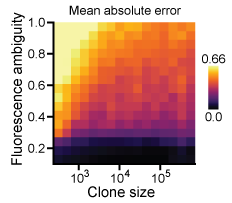
\includegraphics[width=0.9\columnwidth]{./figure_4}
\caption[P:Y ratio is stabilized against varying Pnt and Yan concentrations.]{\textbf{The Pnt-to-Yan ratio is stabilized against varying Pnt and Yan concentrations in progenitor cells.} (A-D) Moving averages of (A, B) Pnt-GFP and (C, D) Yan levels in progenitor and differentiating cells with one (A, C) versus two (B, D) copies of the \textit{pnt-gfp} gene. Measurements used DAPI to mark nuclei. Colors denote cell type. Shaded regions are bootstrapped 95\% confidence intervals for the moving average. (E) Comparison of Pnt-to-Yan ratios between progenitor cells with one versus two copies of \textit{pnt-gfp} during cell fate transitions. Colors denote cell fate transition periods for each R cell type. These time periods are defined in each disc by the times spanned by the first ten identifiable R cells. The concurrent progenitor cell populations are selected from these time windows. Light grey filled boxes denote 1x \textit{pnt-gfp}, dark grey filled boxes denote 2x \textit{pnt-gfp}. Pnt-to-Yan ratios in progenitor cells are indistinguishable between gene dosages during R8, R2/R5, and R1/R6 cell fate transitions (KS 2-sample test, $p<0.001$). (F-G) Confocal image slice of progenitor nuclei in a disc containing loss-of-function \textit{yan} clones. RFP fluorescence marks wildtype \textit{yan}. (H) Quantitative comparison of Pnt-GFP expression between \textit{yan} genotypes. Progenitor cells were assigned \textit{yan} genotypes based on measured RFP level, and Pnt-GFP levels were corrected to account for fluorescence bleed-through (see \ref{ch:clones:correction}). Pnt-GFP levels decrease when no gene copies of \textit{yan} are present (Mann-Whitney \textit{U} tests). Red dots denote the median of each distribution, thick grey lines denote the interquartile range.}
\label{fig:ratio:fig4}
\end{figure}

\section{Notch signaling lowers the Pnt-to-Yan ratio in progenitor cells}

Progenitor cells are dynamically stable about a constant Pnt-to-Yan ratio, but this fixed ratio changes as cells transition to an R cell state. We next asked how the ratio is set in individual cells targeted for differentiation. Notch and RTK signaling provide both transcriptional and post-transcriptional inputs to the Yan-Pnt network \cite{Graham2010}, and therefore present prime candidates to establish and modulate the Pnt-to-Yan ratio. The two pathways generally exert opposing influence on R cell state transitions. Notch signaling is required to maintain progenitor cells in a multipotent state \cite{Fortini1993}, and ensures proper patterning of the first group of R cells by constraining the proximity of adjacent R8 cells \cite{Lubensky2011,Gavish2016}. Conversely, RTK signaling is required to initiate each of the subsequent R cell state transitions \cite{Freeman1996}. Both signaling pathways influence the Pnt-Yan network in multipotent eye cells \cite{Brunner1994,Rebay1995,Rogge1995}. Notch stimulates Yan expression \cite{Rohrbaugh2002}, while RTK activates PntP2 and stimulates PntP1 expression \cite{Brunner1994,Shwartz2013} while attenuating the pulse of Yan expression \cite{Rebay1995,Pelaez2015a}. The precise influence of Notch and RTK signaling on the Pnt-to-Yan ratio are difficult to predict as the two pathways are coupled by feedback within and beyond the Pnt-Yan network \cite{Rohrbaugh2002,Kumar2003,Voas2004}.

We used a temperature-sensitive \textit{Notch} mutant \cite{Cagan1989} to measure the impact of Notch-mediated signaling on Pnt-GFP and Yan. We divided the eye field into two regions for analysis purposes (Fig. \ref{fig:ratio:figS7}A, dashed yellow line). The first region starts anterior to the MF and ends in the region of R8 cell specification. The second region extends $\sim$ 10 columns of R8 cells posterior to the first region. These regions contain the first and second pulses of Pnt-GFP, respectively (Fig. \ref{fig:ratio:figS7}A, thick black lines).

At the non-permissive temperature, progenitor cells had visibly reduced Yan levels (Fig. \ref{fig:ratio:figS7}A,B), consistent with previous reports of Yan expression's dependence on Notch signaling in the developing eye disc \cite{Rohrbaugh2002}. Pnt-GFP levels were also reduced in region 1, but appeared close to normal at later times (Fig. \ref{fig:ratio:figS7}A,B). Attempts to study ratio dynamics in mutant eye discs were challenging. Notch is essential for proper patterning of R8 cells, so the mutant eye discs had distorted spacing of R8 cells at the non-permissive temperature (Fig. \ref{fig:ratio:figS7}C). The irregularity of the intervals between adjacent columns of R8 cells precluded the conversion of spatial position along the anterior-posterior axis to developmental time. As an alternative to our standard quantitative analysis, we visualized the effects of Notch by mapping the pixel-wise difference between Pnt-GFP and Yan to a diverging color scale (Fig. \ref{fig:ratio:fig5}A,B). Direct visualization of the ratio yielded a very similar view of differential Pnt-GFP/Yan expression, but was prone to computational errors imparted by zero-valued pixels. This qualitative analysis was limited to optical sections specifically spanning the progenitor cells.

At the non-permissive temperature, the \textit{Notch} mutant showed a consistently higher Pnt-to-Yan ratio in progenitor cells in region 2 (Fig. \ref{fig:ratio:fig5}A). This observation suggests that Notch signaling maintains a low Pnt-to-Yan ratio in these undifferentiated cells. The known role of Notch in maintaining multipotency in region 2 \cite{Fortini1993} is consistent with our hypothesis that cell state transitions are mediated by the transcription factor ratio.

The Notch mutant revealed more complex behavior in region 1, where the first group of R cell transitions occur. In this region Notch is required for patterning of the R8 lattice \cite{Lubensky2011}. At the permissive temperature, there was a periodic pattern in the Pnt-to-Yan ratio of progenitor cells (Fig. \ref{fig:ratio:fig5}B). Clusters of cells with higher ratio alternated with clusters with lower ratio. We quantified the periodicity of this pattern by evaluating the similarity of ratios between cells as a function of their separation distance (Fig. \ref{fig:ratio:fig5}C). We detected periodic spatial patterns with a constant period of oscillation that was approximately equivalent to the length scale separating adjacent R8 cells (Fig. \ref{fig:ratio:fig5}D,E). Since young R8 cells have elevated Pnt-to-Yan ratios, we infer that periodic clusters of high-ratio progenitor cells give rise to the R8, R2/R5, and R3/R4 cells. At the non-permissive temperature, the Pnt-GFP/Yan pattern was strongly impaired (Fig. \ref{fig:ratio:fig5}B). The ratio was more uniform along the dorso-ventral axis, and while there were modestly detectable oscillations in the ratio, their period was not stable (Fig. \ref{fig:ratio:fig5}F,G).

These results are consistent with the consensus understanding that Notch signaling serves dual roles in R8 fate determination. Initially, Notch pushes clusters of progenitor cells towards an R8 cell state. Later, Notch restricts differentiation to ensure only one cell per cluster adopts an R8 state \cite{Baker1997,Li2001,Lubensky2011}. If Notch signaling is inhibited, very few high Pnt-to-Yan ratio clusters and R8 cells are formed because the first step is blocked \cite{Baker1997}. If cell state transitions are coupled to the Pnt-to-Yan ratio, then the \textit{Notch} mutant would not be expected to have high-ratio clusters in region 1. This is precisely what we observed.

\begin{figure}[h!]
\centering
\includegraphics[width=1.0\columnwidth]{./figure_5}
\caption[Notch signaling lowers the Pnt-to-Yan ratio in progenitor cells.]{ (Continued on the next page.) }
\label{fig:ratio:fig5}
\end{figure}
\begin{figure}[h!]
\contcaption{\textbf{Notch signaling lowers the Pnt-to-Yan ratio in progenitor cells.} (A) Visualization of relative Pnt and Yan expression in progenitor cells in region 2 when Notch signaling is active (left panel) and restricted (right panel). Color scale reflects the difference between Pnt-GFP and Yan fluorescence. Black lines denote periods of elevated Pnt-GFP expression. See methods for details on post-processing of images. (B) Visualization of relative Pnt and Yan expression in progenitor cells during the first wave of cell state transitions. Black arrow marks the morphogenetic furrow. Gold arrows annotate clusters of elevated ratio. (C-E) Quantification of spatial periodicity in the Pnt-to-Yan ratio among progenitor cells immediately posterior to the MF when Notch signaling is active. (C) Spatial correlation functions for progenitor cells in four eye discs. Black lines show the moving average pairwise correlation of Pnt-to-Yan ratios between cells as a function of their separation distance along the dorso-ventral axis. Oscillatory forms indicate alternating regions of similar and dissimilar behavior relative to the population-wide mean. Lines are obtained via first-order Savitzky-Golay filtration with a window size of 50. Shaded region shows a bootstrapped 95\% confidence interval for the moving average. Cell counts are annotated above each correlation function. Red lines are the expected outcome for random expression (no pattern). (D) Normalized Lomb-Scargle periodograms for each disc. Spectra are constructed from individual progenitor cell measurements for periods ranging 50 to 200 px. Grey lines denote spectral power attributed to each oscillation period. Dashed red significance thresholds are obtained by bootstrap resampling the ratio intensities. Asterisks denote signal frequencies exceeding the confidence threshold. In all discs, a pattern in Pnt-to-Yan ratios repeats on a length scale of 73-82 px when Notch signaling is active. (E) Distribution of dorso-ventral separation distances between adjacent R8 neurons within a single column of ommatidia within each disc. Mean values are comparable to the detected oscillation periods. (F,G) No periodicity is detected above the significance threshold when Notch signaling is restricted.}
\end{figure}

\section{Ras signaling elevates the Pnt-to-Yan ratio in progenitor cells}

RTK signals received by progenitor cells trigger their transition to R cell states \cite{Freeman1996}. We quantitatively probed the effect of RTK signaling on Pnt-GFP dynamics and the Pnt-to-Yan ratio by using a temperature-sensitive $EGFR^{ts}$ allele that restricts RTK signaling \cite{Kumar1998}. At high temperatures, the mutant blocks RTK signal transduction, which triggers cell death and allows only R8 neuron patterning. However, animals raised at intermediate temperatures achieve normal recruitment of R8, R2/R5, and R3/R4 neurons, but fail to recruit most R1/R6 and R7 cells \cite{Pelaez2015a}.

At intermediate temperatures, the entire second pulse of Pnt-GFP expression disappeared upon restriction of EGFR activity (Fig. \ref{fig:ratio:figS8}A). Because the second pulse can be predominantly ascribed to PntP2 expression (Fig. \ref{fig:ratio:fig1}I), this result conflicts with a report that PntP2 expression is not dependent upon RTK signaling \cite{Shwartz2013}. At intermediate signaling, Yan levels were also reduced, resulting in Pnt-to-Yan ratios that were indistinguishable from wildtype during the second wave of state transitions (Fig. \ref{fig:ratio:figS8}B,C).

\begin{figure}[h]
\centering
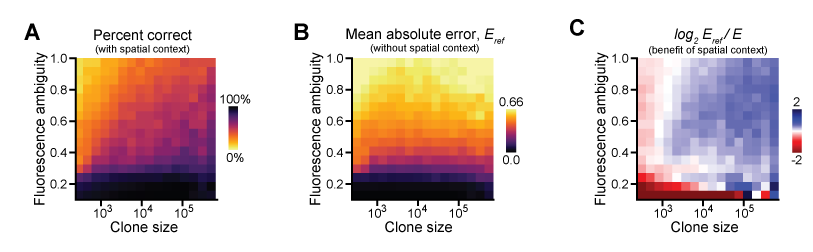
\includegraphics[width=1.0\columnwidth]{./figure_S8}
\caption[Pnt and Yan expression dynamics in $EGFR^{ts}$ eye discs.]{\textbf{Pnt and Yan expression dynamics in $EGFR^{ts}$ eye discs.} (A-C) Effects of $EGFR^{ts}$ on (A) Pnt-GFP, (B) Yan, and (C) Pnt-to-Yan ratio dynamics in progenitor cells. Lines are moving averages across 250 sequential cells. Shaded regions are bootstrapped 95\% confidence intervals for the mean. Solid lines and grey shading denote wildtype controls. Dashed lines and red shading denote restricted EGFR signaling. Black bars denote second period of elevated Pnt-GFP expression.}
\label{fig:ratio:figS8}
\end{figure}

We next asked whether RTK signaling is sufficient to induce an increase in the Pnt-to-Yan ratio of progenitor cells by expressing a constitutively-active form of Ras \cite{Simon1991,Fortini1992}. This construct uses a \textit{sev} promoter to drive Ras expression, limiting its effects to the second region of Pnt-GFP expression. Constitutive Ras activity dramatically increased the amplitude and duration of the second pulse of Pnt-GFP expression in progenitor cells (Fig. \ref{fig:ratio:fig6}A) but did not significantly alter Yan expression dynamics (Fig. \ref{fig:ratio:fig6}B). This yielded a sustained increase in Pnt-to-Yan ratio in progenitors during the second wave of state transitions (Fig. \ref{fig:ratio:fig6}C), as well as the ectopic differentiation of R cells. As previously reported \cite{Fortini1992}, supernumerary cells included extra R7 cells, as well as additional R cells whose identities were not discerned due to their aberrant positioning.

We sought to determine whether these ectopic R cells emerged from a pool of progenitors with abnormally high Pnt-to-Yan ratios. Focusing our analysis on progenitor cells concurrent with the ectopic induction of R cells revealed that their ratios were higher than those of wildtype progenitor cells at comparable times (Fig. \ref{fig:ratio:fig6}D,E grey boxes). Nearly all young supernumerary R cells had ratios that were within the range of mutant progenitor cells, and were above the range observed in wildtype cells (Fig. \ref{fig:ratio:fig6}D,E blue and purple markers). These observations suggest that abnormally high Pnt-to-Yan ratios in progenitor cells accompany ectopic R cell state transitions.

\begin{figure}[h!]
\centering
\includegraphics[scale=1.0]{./figure_6}
\caption[Ras signaling elevates the Pnt-to-Yan ratio in progenitor cells.]{\textbf{Ras signaling elevates the Pnt-to-Yan ratio in progenitor cells.} (A-C) Effects of constitutive Ras signaling on (A) Pnt-GFP, (B) Yan, and (C) Pnt-to-Yan ratio dynamics in progenitor cells. Lines are moving averages across 250 sequential cells. Shaded regions are bootstrapped 95\% confidence intervals for the mean. Solid lines and grey shading denote wildtype controls. Dashed lines and red shading denote constitutive Ras signaling by $Sev>Ras^{V12}$. Black bars denote periods of elevated Pnt-GFP expression. We previously reported a modest increase in the duration of Yan-YFP expression in $Sev>Ras^{V12}$. mutant progenitor cells \cite{Pelaez2015a}, but this difference was not detected using the Yan antibody. (D, E) Comparison of Pnt-to-Yan ratios between wildtype and $Sev>Ras^{V12}$ progenitor cells concurrent with the ectopic differentiation of (D) unidentified R cells and (E) R7 cells in $Sev>Ras^{V12}$ discs. Markers denote the first 25 supernumerary R cells.}
\label{fig:ratio:fig6}
\end{figure}

\section{Ratiometric control as a model for cell fate commitment}

Successful cell state transitions usually require changes in mRNA and protein expression, which are often dictated by transcription factors. It is widely believed that expression depends on the absolute concentration of these factors \cite{Spitz2012}. We have identified a scenario in which cells respond to the ratio in abundance of two transcription factors rather than to the absolute concentration of either protein. This novel mechanism is made possible by several characteristics of the system. First, target genes of these factors are induced when cells transit to differentiated states, and expression of these targets is necessary for differentiation \cite{Xu2000,Nagaraj2002}. Second, both factors bind to the same DNA sites in their target genes. Third, they exert opposing effects on transcription.

A theoretical analysis reveals that, under these conditions, relative site occupancy by either factor determines whether or not a target gene is transcribed. When binding sites are saturated, the probability a site is occupied by one of the factors is controlled by the ratio of factor concentrations and not by the absolute concentration of the factors. This mechanism allows the transcription factors to have pulsatile expression dynamics and still consistently regulate transcription. Regulation of genes through pulsatile dynamics of competing transcription factors with opposing effects has been reported in yeast \cite{Lin2015}. In the developing eye, however, this competition relies on the ratio of the two factors to differentially regulate genes. Perhaps the pulsatile dynamics of Pnt and Yan allow R cell state transitions to be restricted to a specific period of developmental time.

We developed a model to demonstrate that stabilizing interactions between adjacently bound monomers can sensitize enhancer occupancy to the relative abundance of two competing transcription factors. The model does not offer a rigorous characterization of the competition between Pnt and Yan for a specific enhancer, as the data required to construct such a model are not available. For example, it is unknown whether nuclear concentrations of Pnt and Yan protein are of an equivalent order of magnitude in differentiating eye cells. Similarly, we do not know the strength, number, or arrangement of bindings sites in the enhancers targeted by Pnt and Yan. However, the conclusions we have drawn from our model do not rely upon specific values for these variables, and are consequently not anchored to the specific details of any one system. 

In general, the proposed ratiometric sensing mechanism is well suited when either or both transcription factors bind their target sites in a manner stabilized by cooperative interactions. Like its human ortholog TEL1 \cite{Kim2001}, DNA-bound Yan monomers enhance recruitment of Yan to adjacent binding sites through stabilizing SAM-SAM polymerization \cite{Zhang2010}. We show theoretically that such cooperativity could generate threshold-like behavior and cause ultrasensitive switching in site occupancy between Yan and Pnt. In this model, the switching is agnostic to the absolute abundance of either transcription factor as long as their relative ratio can be precisely controlled. This mechanism would enable state transitions to proceed despite variation in protein concentrations driven by fluctuations in metabolism, cell volume, expression noise, environmental conditions, genetic polymorphisms, or gene copy number.

The average Pnt-to-Yan ratio is dynamically stable about an approximately constant value within each cellular state, and only exhibits transient fluctuations when cells switch states. These dynamics reflect the capacity of the system to coordinate the relative expression of the two transcription factors. We have found that the abundance of each transcription factor depends upon the expression of the other factor. Dependencies of this type are often depicted as positive or negative regulation in cartoons of qualitative regulatory interactions (Fig. \ref{fig:ratio:fig7}A). We believe that as biology becomes increasingly quantitative it will be more fruitful to emphasize an empirical description of system dynamics based on control theory (Fig. \ref{fig:ratio:fig7}B).

From a control perspective, a system of cellular components monitors the relative abundance of Pnt and Yan and takes corrective action when the ratio deviates from a specified reference value. The particular components responsible for implementing control may remain unspecified. This perspective eschews molecular events in favor of minimizing complexity, but preserves the salient features of a detailed molecular mechanism and can enable quantitative predictions.

Fluctuations in the absolute abundance of one factor are mitigated by compensatory adjustment of the other. Notch or RTK activity could modulate Pnt or Yan protein levels to transiently perturb the Pnt-to-Yan ratio (Fig. \ref{fig:ratio:fig7}B, dashed black arrow). These signals could permanently set the ratio by adjusting the reference value (Fig. \ref{fig:ratio:fig7}B, dashed red arrow). We advocate this control theoretic perspective because it more accurately conveys the fundamental strategy underlying system behavior. Furthermore, accurate model predictions would only require the evaluation of a small number of parameters that characterize Pnt-to-Yan ratio dynamics, obviating the need for experimental measurement of reaction rates during R cell specification in \textit{Drosophila}.

\begin{figure}[h!]
\centering
\includegraphics[scale=1.0]{./figure_7}
\caption[Conceptual models for regulation of the Pnt-to-Yan ratio.]{\textbf{Conceptual models for regulation of the Pnt-to-Yan ratio.} (A) Cartoon of qualitative regulatory interactions suggests Pnt and Yan protein levels are coupled by reciprocal positive feedback (solid lines), while Notch and Ras signaling adjust the Pnt-to-Yan ratio by modulating the levels of each protein (dashed lines). (B) Block diagram of ratio control in the Pnt-Yan network. Lines represent values, rectangles indicate functions, and the circle is a comparison point. The Pnt-to-Yan ratio is compared against a basal reference value, and the difference is fed into a regulatory network that acts to drive the ratio back toward the reference value. Extracellular signals transiently perturb the ratio by modulating Pnt or Yan protein levels (dashed black line), or set the ratio by adjusting the reference value (dashed red line).}
\label{fig:ratio:fig7}
\end{figure}

We have shown that dynamic changes in the Pnt-to-Yan ratio are coupled to cell state. Our favored interpretation is that the ratio determines which state a cell is in. Direct testing of this hypothesis remains difficult because the observed ratio control strategy precludes gene-level manipulation of the ratio. Instead, we acknowledge that our observations are correlative. We cannot discard the possibility that Notch and RTK signaling regulate state transitions in a manner that is not only mediated by the Pnt-to-Yan ratio but by other mechanisms as well. We emphasize, however, that ratio control enforces stability when cells are in one state, which implicates the ratio as an active cell state determinant. Moreover, qualitatively different approaches to experimentally manipulate the ratio affected cell state transitions in a consistent manner. Both Notch inhibition and Ras activation increase the ratio and cause abnormal R cell state transitions \cite{Fortini1992,Yang2006}. Single-cell dynamical measurements of Yan and specific Pnt isoforms during isoform-specific perturbations may ultimately prove necessary to determine definitively whether ratios directly mediate transitions. The regulatory mechanism described here provides insight into how the relative dynamics of competing transcription factors can be used to pattern complex epithelia, and may also aid design of synthetic regulatory systems based on ratiometric sensing.
